\chapter{Results and Discussion}
\label{chap:results}

The experimental evidence is organised around two complementary
lines of investigation. The first examines whether QCLand is competitive
with established landmark-localisation methods across fetal
measurements and dataset settings. The second examines which
architectural and training choices were most consequential in
developing the final QCLand configuration. Comparative results are therefore presented
first, followed by the BPD ablation study and a broader discussion of
the variation, limitations, and implications revealed by both lines
of evidence.


% =================================================================
% 5.1 Comparative Results with State-of-the-Art Methods
% =================================================================

\section{Comparative Results with State-of-the-Art Methods}
\label{sec:results-comparative}
\label{sec:results-track-b}

QCLand-DINOv2 and QCLand-DINOv3 are compared with HRNet-W18 and
RTMPose-s across five fetal measurements on the UCL and Multicentre
datasets. All results use the harmonised evaluation protocol
established in Chapter 4.


\subsection{Overall Performance Across Datasets and Measurements}
\label{sec:results-overall}
\label{sec:results-cross-anatomy}
\label{sec:results-hrnet512}

The overall pattern is clear despite substantial variation across
measurements. QCLand-DINOv3 achieves the lowest five-seed mean PI-NME
on all five UCL measurements, whereas the Multicentre ranking depends
more strongly on anatomy. Across both datasets, a QCLand variant
records the lowest mean error in eight of the ten evaluation settings.
The two exceptions are Multicentre BPD and OFD, where HRNet-W18
records the lowest mean.

\begin{table}[htbp]
  \centering
  \caption{Original-image-space PI-NME (\%), five-seed mean
    $\pm$ sample SD, on the common image subset per setting. Lower is
    better; bold marks the lowest mean per row.}
  \label{tab:four-model-main}
  \label{tab:eomt-track-b}
  \small
  \setlength{\tabcolsep}{4pt}
  \begin{tabular}{llrrrrr}
    \toprule
    \multirow{2}{*}{Dataset} & \multirow{2}{*}{Task} &
      \multicolumn{2}{c}{QCLand} & \multicolumn{2}{c}{Baselines} &
      \multirow{2}{*}{$n$} \\
    \cmidrule(lr){3-4}\cmidrule(lr){5-6}
      & & DINOv2 & DINOv3 & HRNet-W18 & RTMPose-s & \\
    \midrule
    \multirow{5}{*}{UCL}
      & BPD  & 5.92 $\pm$ 0.66 & \textbf{5.14 $\pm$ 0.61} & 5.51 $\pm$ 0.46 & 11.31 $\pm$ 0.86 & 49 \\
      & OFD  & 3.94 $\pm$ 0.55 & \textbf{3.75 $\pm$ 0.09} & 4.59 $\pm$ 0.49 & 9.12 $\pm$ 1.60  & 49 \\
      & APAD & 6.50 $\pm$ 1.15 & \textbf{5.34 $\pm$ 0.66} & 7.33 $\pm$ 1.30 & 16.56 $\pm$ 0.91 & 36 \\
      & TAD  & 9.32 $\pm$ 1.33 & \textbf{6.47 $\pm$ 0.86} & 6.74 $\pm$ 0.98 & 18.98 $\pm$ 1.76 & 36 \\
      & FL   & 1.61 $\pm$ 0.11 & \textbf{1.53 $\pm$ 0.15} & 1.99 $\pm$ 0.41 & 17.83 $\pm$ 1.53 & 39 \\
    \midrule
    \multirow{5}{*}{Multicentre}
      & BPD  & 6.90 $\pm$ 0.17 & 6.09 $\pm$ 0.19 & \textbf{4.68 $\pm$ 0.17} & 6.15 $\pm$ 0.15 & 1180 \\
      & OFD  & 6.13 $\pm$ 0.45 & 5.73 $\pm$ 0.68 & \textbf{4.78 $\pm$ 0.17} & 5.66 $\pm$ 0.10 & 1189 \\
      & APAD & \textbf{6.99 $\pm$ 0.23} & 7.11 $\pm$ 0.21 & 8.89 $\pm$ 0.19 & 8.89 $\pm$ 0.37 & 161 \\
      & TAD  & 8.82 $\pm$ 0.90 & \textbf{8.71 $\pm$ 0.54} & 8.75 $\pm$ 0.33 & 9.22 $\pm$ 0.32 & 161 \\
      & FL   & 2.78 $\pm$ 0.11 & \textbf{2.71 $\pm$ 0.13} & 2.93 $\pm$ 0.32 & 4.95 $\pm$ 0.49 & 362 \\
    \bottomrule
  \end{tabular}
\end{table}

\begin{figure}[htbp]
  \centering
  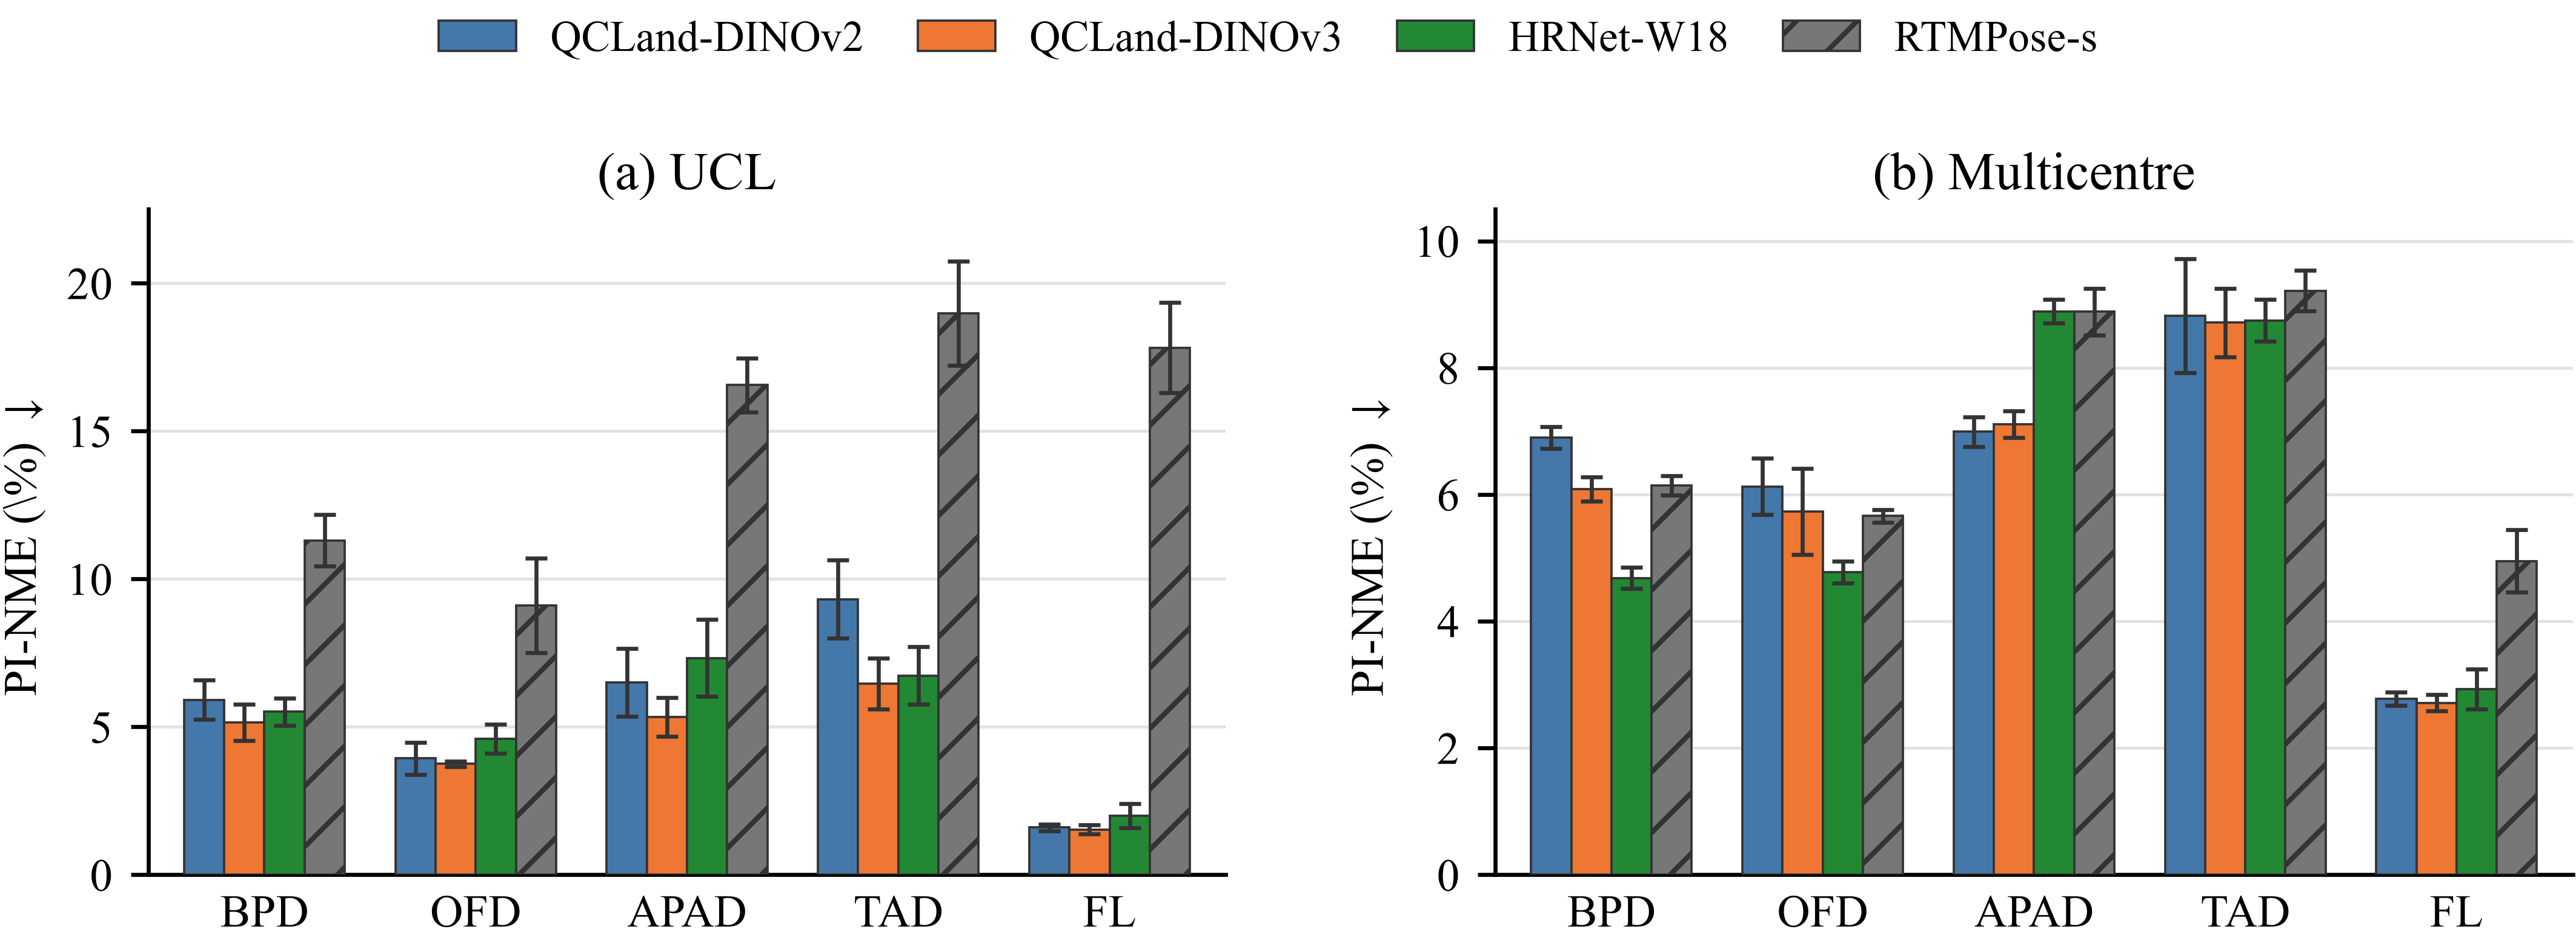
\includegraphics[width=\textwidth]
    {figures/final_four_model_comparison.png}
  \caption{Final four-model comparison across the UCL and Multicentre
    evaluation settings. Bars show five-seed mean PI-NME and error
    bars show the seed-level sample standard deviation for each fetal
    measurement. Lower PI-NME indicates better localisation
    performance. The two panels use different vertical scales for
    readability.}
  \label{fig:four-model-bar}
\end{figure}

The eight-of-ten ranking provides a concise descriptive summary of
QCLand's competitiveness, but it does not imply that every numerical
advantage is statistically supported. The paired analysis therefore
distinguishes descriptive rankings from confirmed differences.


\subsection{Effect of Backbone Choice}
\label{sec:results-backbone}

QCLand-DINOv3 has a lower mean PI-NME than QCLand-DINOv2 in nine of
the ten evaluation settings. The only reversal is Multicentre APAD,
where DINOv2 records 6.99\% and DINOv3 7.11\%. The directional
pattern therefore consistently favours DINOv3 at the descriptive
level.

Inferential support is more limited. None of the five UCL
DINOv2--DINOv3 contrasts reaches Holm-60 Wilcoxon significance.
APAD and TAD have bootstrap intervals that exclude zero without
corresponding Wilcoxon support and are therefore treated as
test-discordant rather than confirmed effects. On Multicentre, BPD
and OFD are supported by both analyses ($p<0.001$), whereas the other
three measurements are not.

The evidence therefore favours DINOv3 descriptively across most
settings but does not support a blanket claim that the newer backbone
is superior for every fetal landmark-localisation task.


\subsection{Comparison with HRNet-W18 and RTMPose-s}
\label{sec:results-baselines}

The paired contrasts are reported in
\Cref{tab:ucl-paired,tab:multicentre-paired}. The discussion below
focuses on the main patterns rather than repeating every numerical
entry.

\paragraph{QCLand versus HRNet-W18.}
On UCL, QCLand and HRNet-W18 are largely comparable. The only
contrast supported by both analyses is TAD with QCLand-DINOv2, for
which QCLand performs worse than HRNet-W18. QCLand-DINOv3 on the
same measurement is statistically indistinguishable from HRNet-W18.
Both QCLand variants show Wilcoxon-supported advantages on FL, but
their bootstrap intervals cross zero.

The Multicentre results are more anatomy-dependent. HRNet-W18
outperforms both QCLand variants on BPD and OFD with agreement between
the bootstrap and Wilcoxon analyses. QCLand, by contrast, outperforms
HRNet-W18 on APAD for both backbones. FL again provides rank-based
support for QCLand without bootstrap confirmation, while TAD shows no
supported difference. Neither architecture therefore dominates
uniformly across anatomical measurements.

\paragraph{QCLand versus RTMPose-s.}
On UCL, both QCLand backbones outperform RTMPose-s on every
measurement, with particularly large differences for FL and the
abdominal measurements.

RTMPose-s is more competitive on Multicentre. QCLand significantly
outperforms it on APAD and FL, while TAD shows no supported
difference. On BPD and OFD, QCLand-DINOv2 performs worse than
RTMPose-s, whereas the DINOv3 backbone substantially narrows this gap.
The evidence therefore does not support a universal advantage of
heatmap-based spatial decoding over coordinate classification.

\begin{table}[htbp]
  \centering
  \caption{UCL paired contrasts (QCLand vs.\ baselines). Differences
    are in percentage points; negative values favour QCLand.}
  \label{tab:ucl-paired}
  \footnotesize
  \setlength{\tabcolsep}{4pt}
  \renewcommand{\arraystretch}{0.92}
  \begin{tabular}{llrrl}
    \toprule
    Task & Contrast & Diff., pp & 95\% CI & Holm-60 $p$ \\
    \midrule
    \multirow{4}{*}{BPD}
      & DINOv2 $-$ HRNet-W18   & 0.41  & [$-$0.98, 1.67]       & 0.081 \\
      & DINOv2 $-$ RTMPose-s   & $-$5.39 & [$-$7.63, $-$3.34] & $<$0.001 \\
      & DINOv3 $-$ HRNet-W18   & $-$0.37 & [$-$1.77, 0.76]    & 0.219 \\
      & DINOv3 $-$ RTMPose-s   & $-$6.16 & [$-$8.51, $-$4.00] & $<$0.001 \\
    \cmidrule(lr){2-5}
    \multirow{4}{*}{OFD}
      & DINOv2 $-$ HRNet-W18   & $-$0.65 & [$-$1.78, 0.16]    & 0.861 \\
      & DINOv2 $-$ RTMPose-s   & $-$5.18 & [$-$7.25, $-$3.37] & $<$0.001 \\
      & DINOv3 $-$ HRNet-W18   & $-$0.84 & [$-$2.19, 0.07]    & 1.000 \\
      & DINOv3 $-$ RTMPose-s   & $-$5.36 & [$-$7.50, $-$3.49] & $<$0.001 \\
    \cmidrule(lr){2-5}
    \multirow{4}{*}{APAD}
      & DINOv2 $-$ HRNet-W18   & $-$0.83 & [$-$3.12, 1.25]    & 1.000 \\
      & DINOv2 $-$ RTMPose-s   & $-$10.06 & [$-$13.35, $-$7.23] & $<$0.001 \\
      & DINOv3 $-$ HRNet-W18   & $-$1.99 & [$-$4.80, 0.51]    & 1.000 \\
      & DINOv3 $-$ RTMPose-s   & $-$11.22 & [$-$14.94, $-$8.16] & $<$0.001 \\
    \cmidrule(lr){2-5}
    \multirow{4}{*}{TAD}
      & DINOv2 $-$ HRNet-W18   & 2.58  & [0.42, 5.16]          & 0.035 \\
      & DINOv2 $-$ RTMPose-s   & $-$9.66 & [$-$14.99, $-$4.93] & 0.005 \\
      & DINOv3 $-$ HRNet-W18   & $-$0.27 & [$-$2.80, 2.20]    & 0.474 \\
      & DINOv3 $-$ RTMPose-s   & $-$12.51 & [$-$16.51, $-$8.99] & $<$0.001 \\
    \cmidrule(lr){2-5}
    \multirow{4}{*}{FL}
      & DINOv2 $-$ HRNet-W18   & $-$0.39 & [$-$2.11, 0.55]    & $<$0.001 \\
      & DINOv2 $-$ RTMPose-s   & $-$16.22 & [$-$26.67, $-$8.91] & $<$0.001 \\
      & DINOv3 $-$ HRNet-W18   & $-$0.46 & [$-$2.20, 0.51]    & 0.004 \\
      & DINOv3 $-$ RTMPose-s   & $-$16.29 & [$-$26.65, $-$9.07] & $<$0.001 \\
    \bottomrule
  \end{tabular}
  \par\smallskip
  {\footnotesize Intervals are 95\% paired-bootstrap CIs; $p$ is
    globally Holm-60 adjusted. DINOv2--DINOv3 and HRNet--RTMPose-s
    contrasts are available in the frozen statistical records.}
\end{table}

\begin{table}[htbp]
  \centering
  \caption{Multicentre paired contrasts (QCLand vs.\ baselines).
    Differences are in percentage points; negative values favour
    QCLand.}
  \label{tab:multicentre-paired}
  \footnotesize
  \setlength{\tabcolsep}{4pt}
  \renewcommand{\arraystretch}{0.92}
  \begin{tabular}{llrrl}
    \toprule
    Task & Contrast & Diff., pp & 95\% CI & Holm-60 $p$ \\
    \midrule
    \multirow{4}{*}{BPD}
      & DINOv2 $-$ HRNet-W18   & 2.21  & [1.90, 2.52]          & $<$0.001 \\
      & DINOv2 $-$ RTMPose-s   & 0.75  & [0.41, 1.08]          & $<$0.001 \\
      & DINOv3 $-$ HRNet-W18   & 1.40  & [1.13, 1.67]          & $<$0.001 \\
      & DINOv3 $-$ RTMPose-s   & $-$0.06 & [$-$0.39, 0.24]    & 0.016 \\
    \cmidrule(lr){2-5}
    \multirow{4}{*}{OFD}
      & DINOv2 $-$ HRNet-W18   & 1.35  & [0.98, 1.75]          & $<$0.001 \\
      & DINOv2 $-$ RTMPose-s   & 0.47  & [0.12, 0.82]          & $<$0.001 \\
      & DINOv3 $-$ HRNet-W18   & 0.96  & [0.63, 1.30]          & $<$0.001 \\
      & DINOv3 $-$ RTMPose-s   & 0.07  & [$-$0.23, 0.38]      & 1.000 \\
    \cmidrule(lr){2-5}
    \multirow{4}{*}{APAD}
      & DINOv2 $-$ HRNet-W18   & $-$1.90 & [$-$2.71, $-$1.15] & $<$0.001 \\
      & DINOv2 $-$ RTMPose-s   & $-$1.89 & [$-$2.91, $-$1.03] & $<$0.001 \\
      & DINOv3 $-$ HRNet-W18   & $-$1.78 & [$-$2.53, $-$1.08] & 0.005 \\
      & DINOv3 $-$ RTMPose-s   & $-$1.78 & [$-$2.62, $-$1.02] & $<$0.001 \\
    \cmidrule(lr){2-5}
    \multirow{4}{*}{TAD}
      & DINOv2 $-$ HRNet-W18   & 0.07  & [$-$0.74, 0.89]       & 1.000 \\
      & DINOv2 $-$ RTMPose-s   & $-$0.40 & [$-$1.75, 0.76]    & 1.000 \\
      & DINOv3 $-$ HRNet-W18   & $-$0.04 & [$-$0.69, 0.63]    & 1.000 \\
      & DINOv3 $-$ RTMPose-s   & $-$0.50 & [$-$1.96, 0.66]    & 1.000 \\
    \cmidrule(lr){2-5}
    \multirow{4}{*}{FL}
      & DINOv2 $-$ HRNet-W18   & $-$0.15 & [$-$0.74, 0.30]    & $<$0.001 \\
      & DINOv2 $-$ RTMPose-s   & $-$2.17 & [$-$5.00, $-$0.59] & $<$0.001 \\
      & DINOv3 $-$ HRNet-W18   & $-$0.22 & [$-$0.82, 0.23]    & $<$0.001 \\
      & DINOv3 $-$ RTMPose-s   & $-$2.24 & [$-$5.16, $-$0.56] & $<$0.001 \\
    \bottomrule
  \end{tabular}
  \par\smallskip
  {\footnotesize Intervals are 95\% paired-bootstrap CIs; $p$ is
    globally Holm-60 adjusted. DINOv2--DINOv3 and HRNet--RTMPose-s
    contrasts are available in the frozen statistical records.}
\end{table}


\subsection{Interpretation of the Comparative Results}
\label{sec:discussion-comparative}
\label{sec:discussion-significance}

Taken together, the comparative evidence supports the central claim
behind RQ1 and RQ3: query-conditioned foundation-model
representations can be adapted effectively to precise fetal landmark
localisation, but their advantage is not invariant to anatomy or
dataset setting.

The clearest distinction from HRNet-W18 lies in the anatomical
pattern. QCLand is strongest on the abdominal measurements and remains
competitive on FL, whereas HRNet-W18 retains a clear advantage on the
Multicentre head measurements. This suggests that the value of
pretrained transformer representations and query-conditioned spatial
decoding depends on the geometry and appearance characteristics of the
target measurement rather than uniformly replacing a convolutional
landmark architecture.

RTMPose-s provides a complementary comparison. Its poor UCL
performance shows that a modern coordinate-classification formulation
does not automatically transfer well to these relatively small fetal
datasets. Its stronger Multicentre performance, particularly on the
head measurements, nevertheless prevents a general conclusion that
dense heatmap decoding is inherently superior to coordinate
classification.

The DINOv2--DINOv3 comparison follows the same pattern of qualified
evidence. DINOv3 records the lower mean in nine of ten settings, but
paired support is concentrated on Multicentre BPD and OFD. The larger
Multicentre samples may make smaller differences easier to detect, but
the present experiments do not include a matched subsampling analysis
capable of separating statistical power from genuinely
dataset-dependent backbone behaviour.


% =================================================================
% 5.2 Results of Ablation Study
% =================================================================

\section{Results of Ablation Study}
\label{sec:results-development}
\label{sec:results-track-a}

The BPD experiments trace the development of the adopted QCLand
configuration and address RQ2. The study includes both controlled
component comparisons and sequential development steps. It is
therefore interpreted as a staged ablation study rather than a fully
factorial decomposition of every component. The target-width
experiment is a single-seed exploratory screen; the subsequent
controlled comparisons use the five predefined seeds unless stated
otherwise.


\subsection{Target Width and Objective Selection}
\label{sec:results-bpd-sigma}
\label{sec:results-bpd-loss}

An initial single-seed experiment (seed 2024) using the original
dot-product readout showed that increasing the Gaussian target width
from $\sigma=1$ to $\sigma=4$ reduced PI-NME from 149.89\% to
50.46\%. This exploratory result motivated the use of $\sigma=4$ in
the subsequent experiments and is not treated as a formal five-seed
comparison.

The training objective was then examined under a controlled five-seed
design while retaining the dot-product readout.

\begin{table}[htbp]
  \centering
  \caption{BPD loss screening, dot-product readout, five-seed
    final-checkpoint PI-NME, mean $\pm$ sample SD, $n=49$.}
  \label{tab:bpd-loss}
  \begin{tabular}{@{}lr@{}}
    \toprule
    Loss & PI-NME \\
    \midrule
    Plain heatmap MSE
      & 36.65 $\pm$ 17.28\% \\
    Weighted heatmap MSE
      & 13.75 $\pm$ 2.90\% \\
    Hybrid (weighted MSE + coordinate L1)
      & 11.23 $\pm$ 2.06\% \\
    \bottomrule
  \end{tabular}
\end{table}

Plain heatmap MSE produced both the highest error and the greatest
seed-to-seed variability. Peak reweighting substantially reduced both,
and adding coordinate supervision produced a further reduction. The
hybrid objective was therefore adopted for all subsequent
experiments.


\subsection{Contribution of DeconvHeadV2 and Feature Fusion}
\label{sec:results-bpd-ablation}

The staged architecture chain is summarised in
\Cref{tab:bpd-progression,fig:bpd-development}. All four
configurations use the hybrid objective, the same five seeds, and the
same PI-NME evaluation.

\begin{table}[htbp]
  \centering
  \caption{BPD architecture development chain, five-seed
    final-checkpoint PI-NME, mean $\pm$ sample SD, $n=49$.}
  \label{tab:bpd-progression}
  \begin{tabular}{@{}lr@{}}
    \toprule
    Configuration & PI-NME \\
    \midrule
    Dot-product readout (baseline)
      & 11.23 $\pm$ 2.06\% \\
    DeconvHeadV2
      & 8.12 $\pm$ 1.42\% \\
    \quad + multi-depth fusion
      & 9.00 $\pm$ 2.20\% \\
    \quad + pixel-centre alignment
      & 8.96 $\pm$ 2.30\% \\
    \bottomrule
  \end{tabular}
\end{table}

\begin{figure}[p]
  \centering
  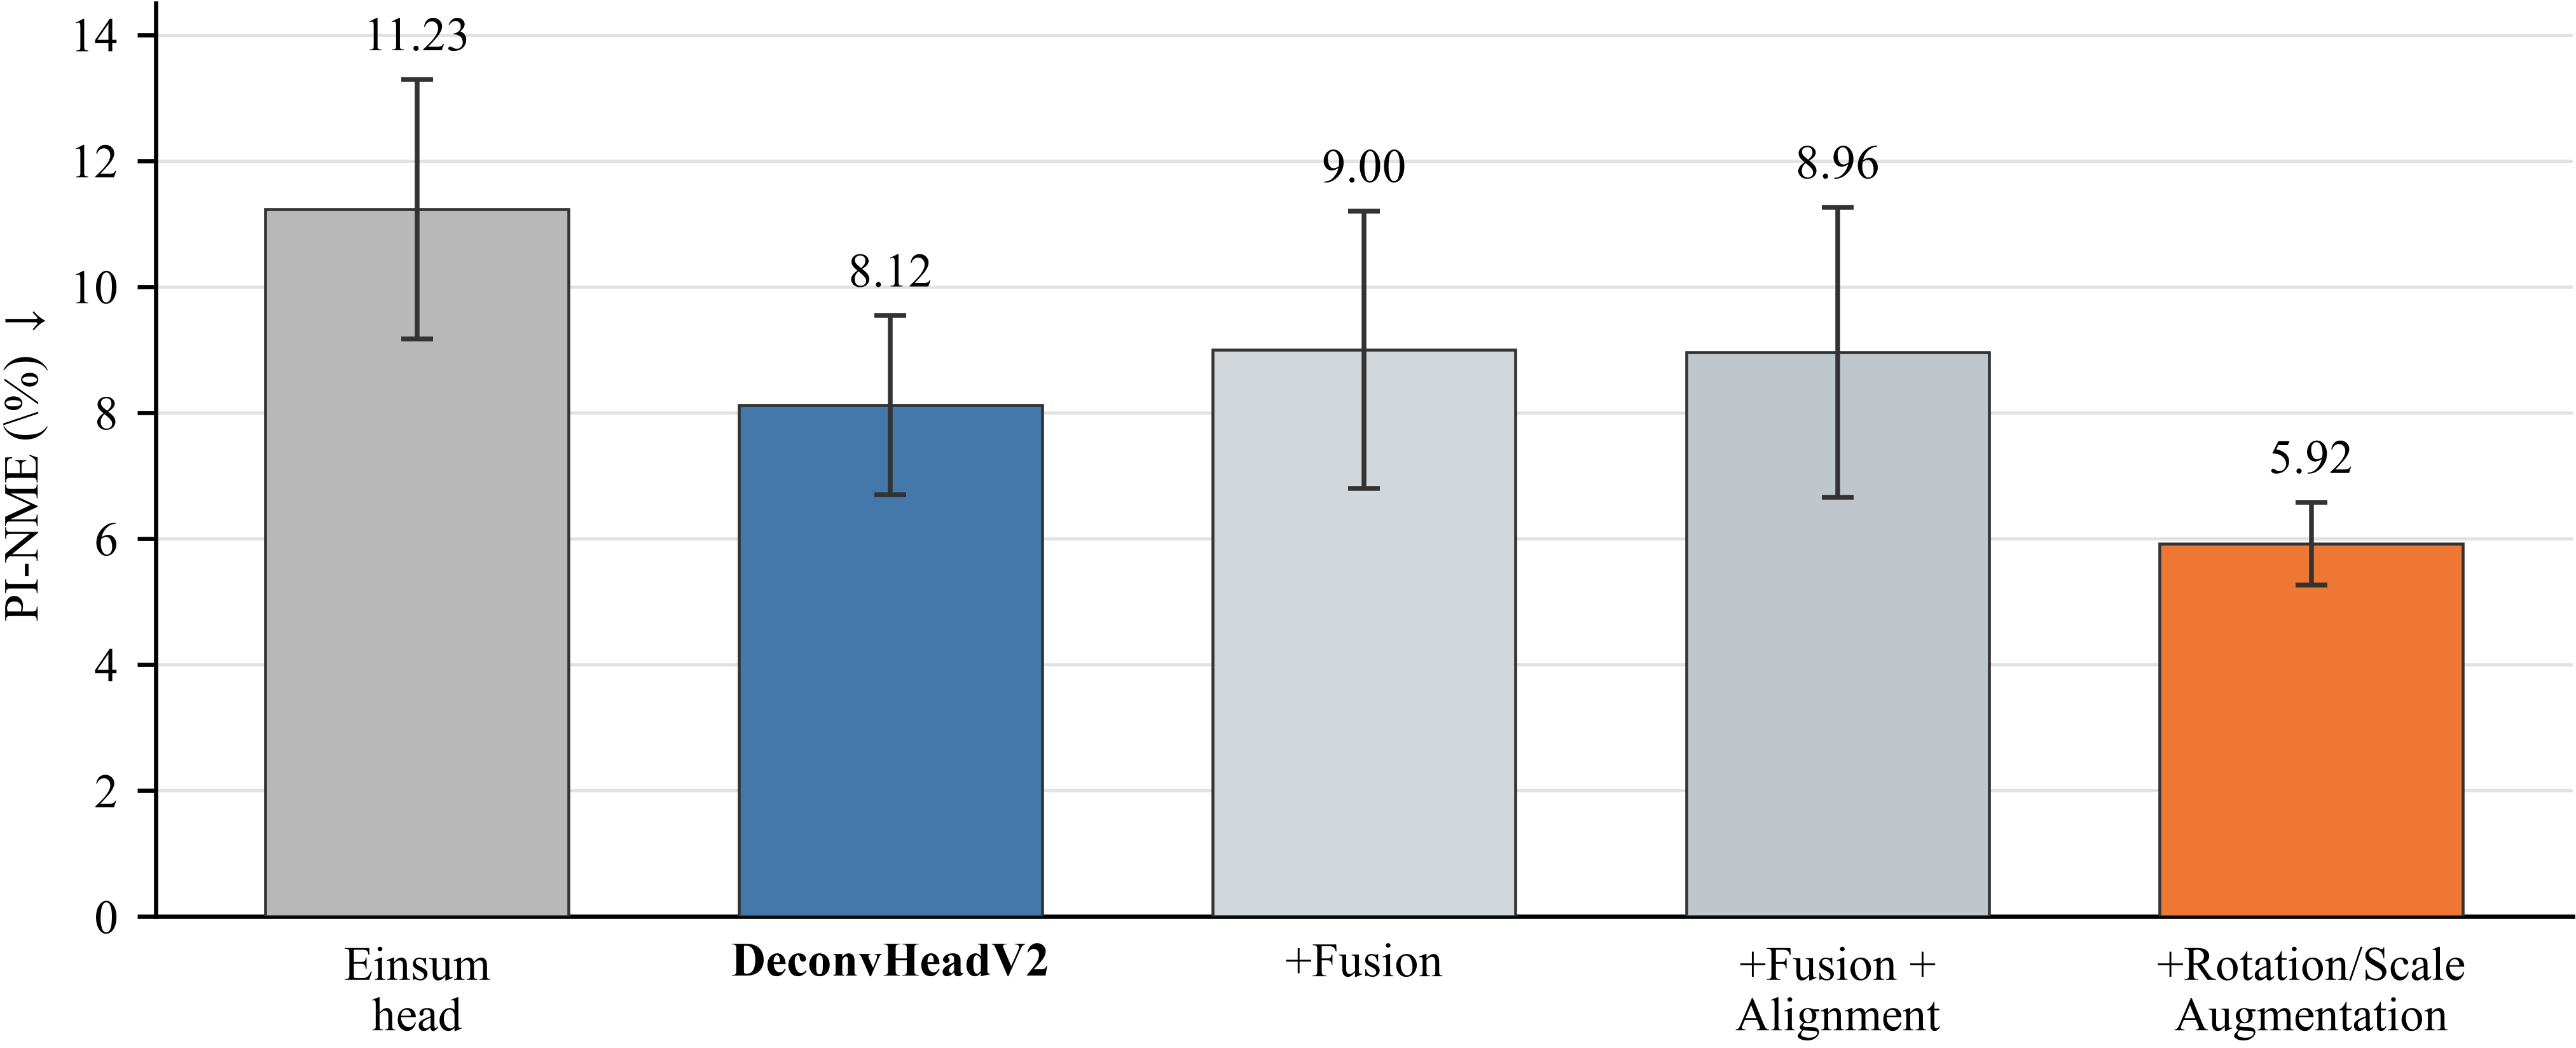
\includegraphics[width=0.95\textwidth]
    {figures/bpd_staged_development.png}
  \caption{Staged BPD ablation results. Bars show five-seed mean
    PI-NME and error bars show seed-level sample SD. The sequence
    represents model development rather than a factorial ablation.}
  \label{fig:bpd-development}

  \vspace{0.8em}

  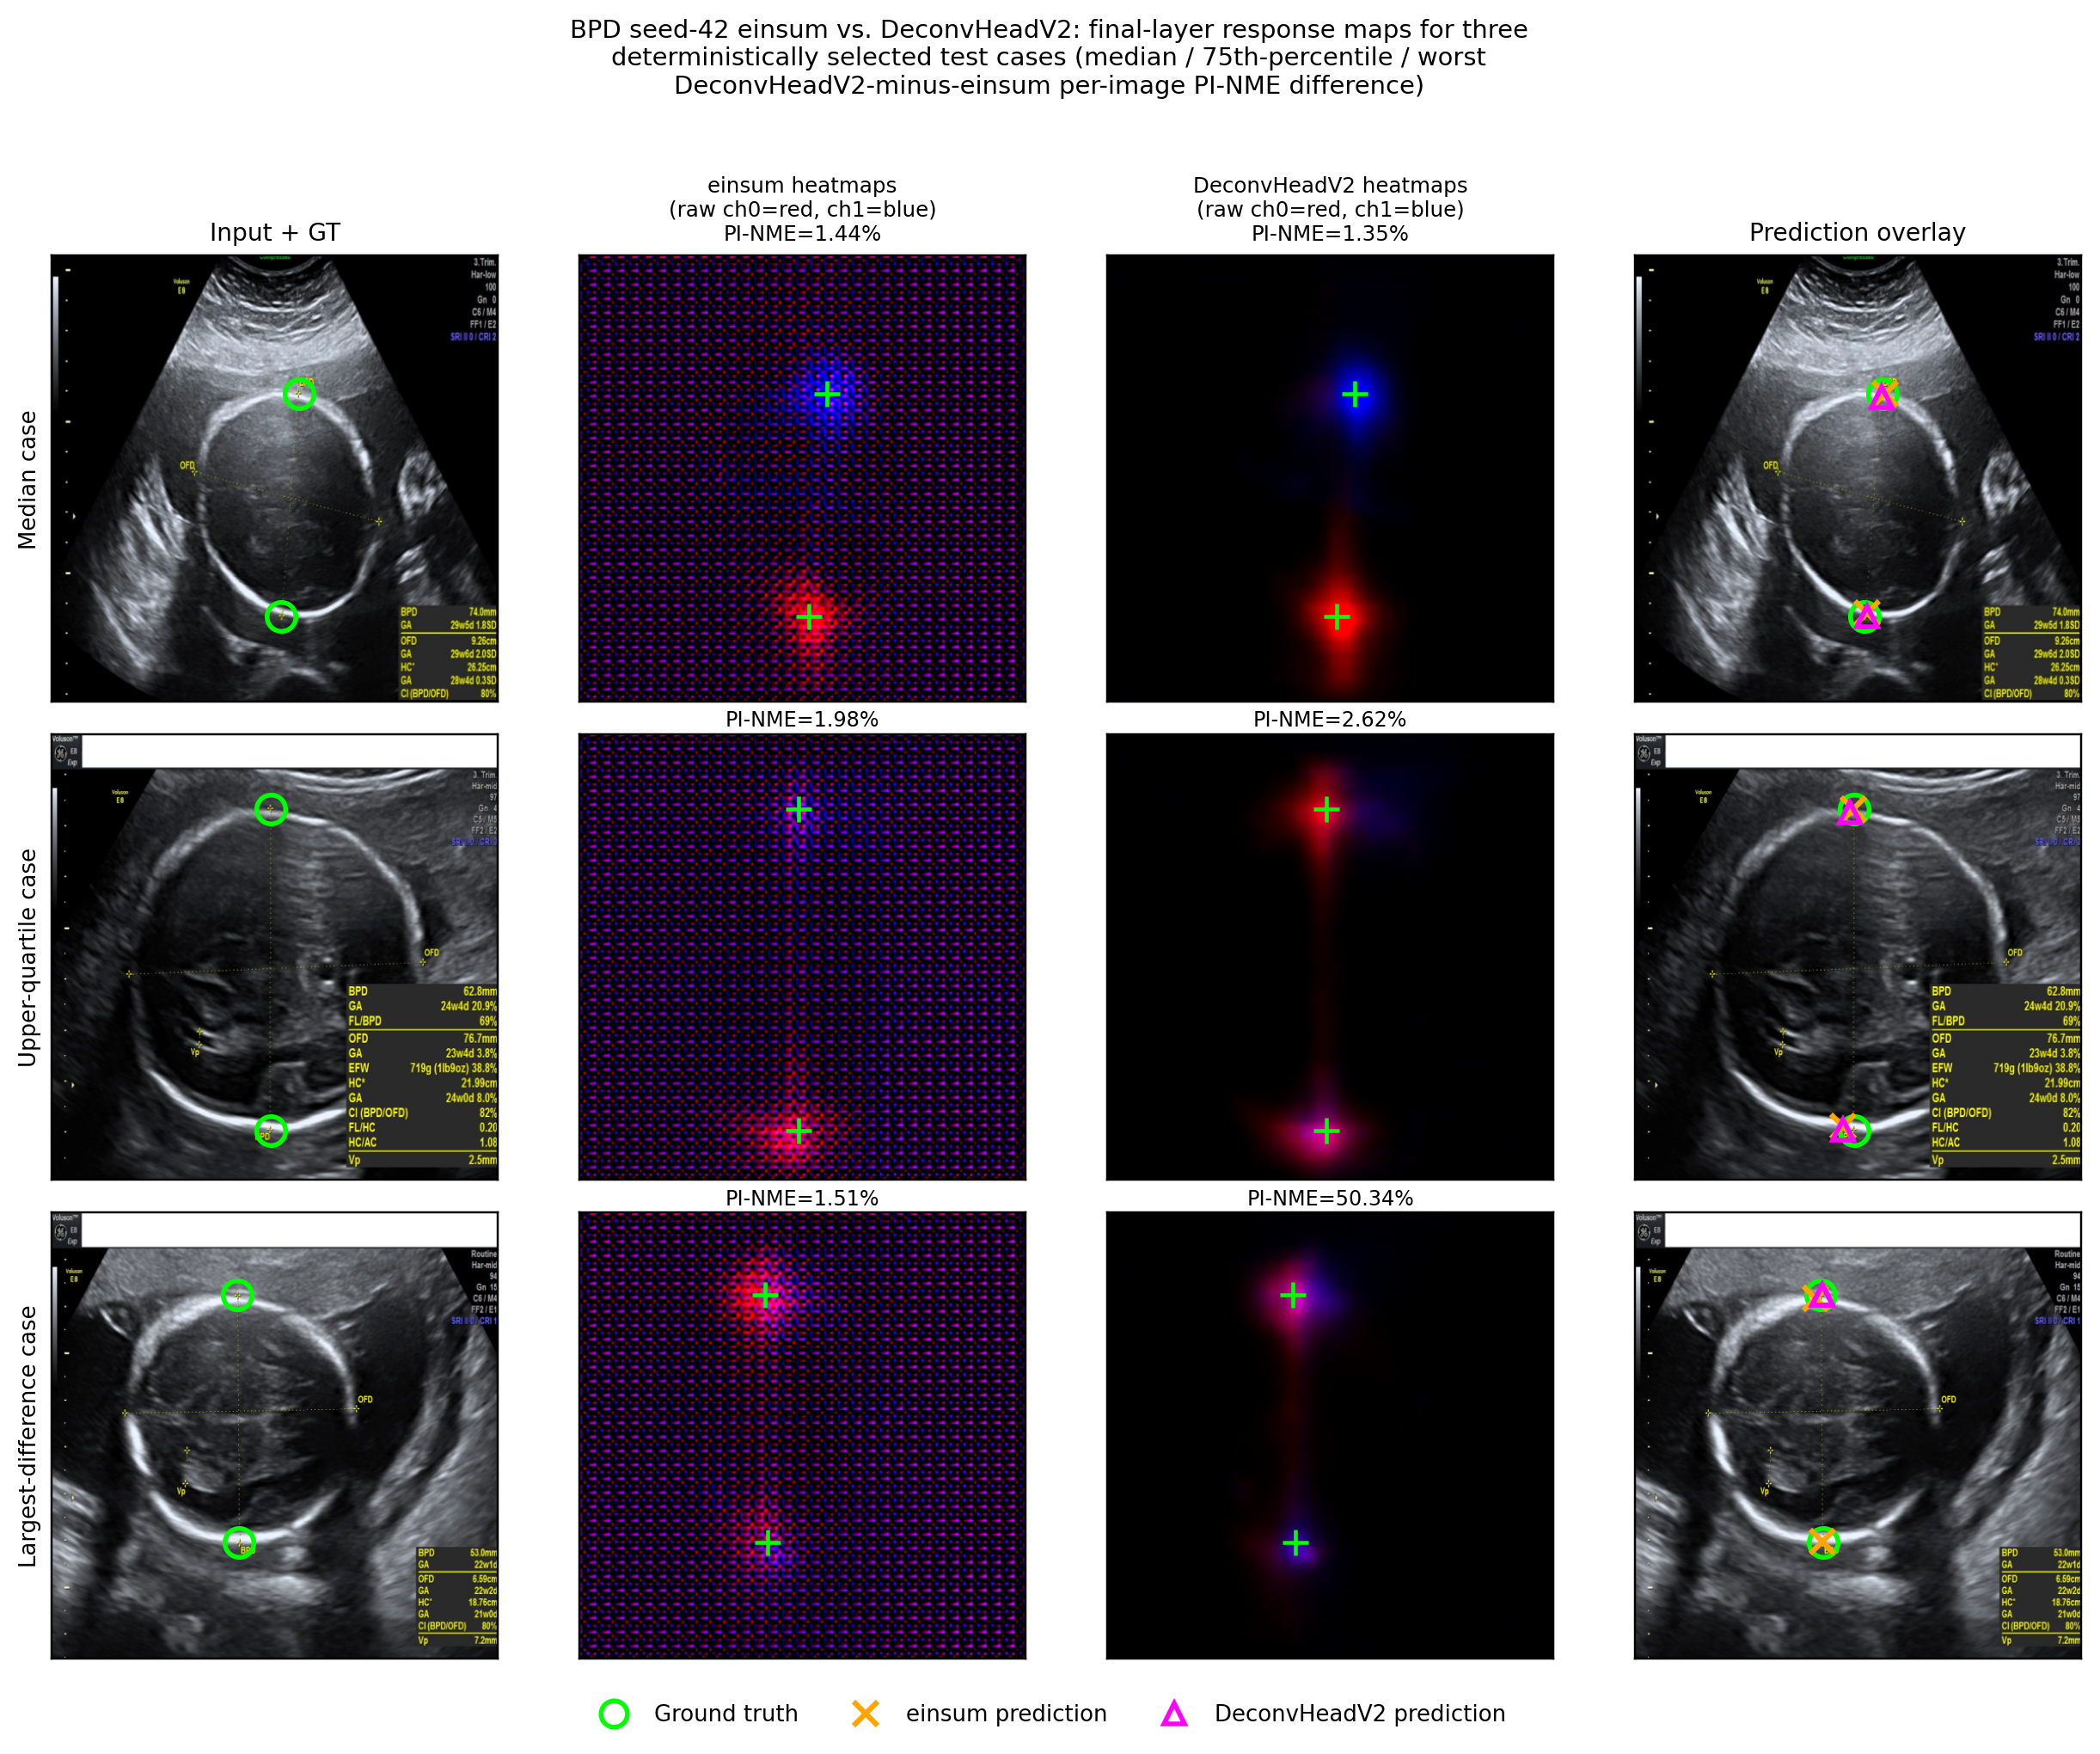
\includegraphics[width=0.95\textwidth]
    {figures/bpd_einsum_deconvheadv2_heatmaps.png}
  \caption[Qualitative readout comparison]{Qualitative comparison of
    the dot-product readout and DeconvHeadV2 on three deterministically
    selected BPD cases (seed 42). Heatmaps show the raw query channels
    (channel 0 red, channel 1 blue); green, orange, and magenta markers
    denote ground truth, dot-product predictions, and DeconvHeadV2
    predictions, respectively. The examples are illustrative rather
    than a statistical sample.}
  \label{fig:einsum-deconvheadv2-heatmaps}
\end{figure}

DeconvHeadV2 produces the largest observed architectural improvement,
reducing PI-NME from $11.23\pm2.06\%$ to $8.12\pm1.42\%$. This is
consistent with its intended role: replacing an independent
per-location dot-product readout with a query-conditioned spatial
decoder capable of local spatial mixing.

Adding multi-depth feature fusion does not further reduce the mean in
the unaugmented chain ($8.12\%\rightarrow9.00\%$), while adding
pixel-centre alignment produces only a small numerical change
($9.00\%\rightarrow8.96\%$). No paired significance tests were
performed between these sequential architecture rungs, so these
differences are interpreted descriptively.

The qualitative comparison provides a complementary view of the
decoder change. In two of the three deterministically selected cases,
DeconvHeadV2 produces visibly more concentrated responses than the
dot-product readout. The remaining case shows both query channels
responding to the same spatial peak, illustrating that the aggregate
improvement does not eliminate all image-level failure modes.


\subsection{Effect of Rotation-and-Scale Augmentation}
\label{sec:results-augmentation}

Rotation-and-scale augmentation is associated with the largest
subsequent reduction in the complete development chain. The
unaugmented complete configuration records $8.96\pm2.30\%$, compared
with $5.92\pm0.66\%$ for the corresponding augmented
QCLand-DINOv2 configuration. The change is accompanied by a
substantial reduction in run-to-run variability.

Because the sequential comparison cannot determine whether this
improvement arises from augmentation alone or from its interaction
with fusion and alignment, a targeted matched follow-up compares
augmented DeconvHeadV2 alone with the complete augmented
configuration.

\begin{table}[htbp]
  \centering
  \caption{BPD augmented-configuration comparison, five-seed
    final-checkpoint PI-NME, mean $\pm$ sample SD, $n=49$.}
  \label{tab:bpd-augmented}
  \begin{tabular}{@{}lr@{}}
    \toprule
    Configuration & PI-NME \\
    \midrule
    DeconvHeadV2 + augmentation
      & 6.30 $\pm$ 0.67\% \\
    DeconvHeadV2 + fusion + alignment + augmentation
      & 5.92 $\pm$ 0.66\% \\
    \bottomrule
  \end{tabular}
\end{table}

The complete configuration has a 0.38 percentage-point lower mean.
The 20{,}000-resample paired-bootstrap confidence interval crosses
zero ($-0.48$ to $+1.28$), whereas the Pratt--Wilcoxon test rejects
its null hypothesis ($p=0.0078$). The bootstrap therefore does not
confirm a non-zero mean difference, while the rank-based analysis
supports a distributional shift. Because fusion and pixel-centre
alignment change together in this contrast, their individual
contributions remain unresolved.


\subsection{Input-Resolution Sensitivity}
\label{sec:results-resolution}

A matched five-seed comparison between $256\times256$ and
$512\times512$ input resolution was conducted using the complete
augmented QCLand-DINOv2 configuration. Heatmap resolution remained
fixed at $64\times64$. The higher-resolution configuration produces a
numerically lower mean and smaller run-to-run spread
($6.61\pm0.91\%$ versus $7.30\pm1.50\%$). No paired significance
test was conducted, so the comparison remains descriptive. The
$512\times512$ result in this experiment is an independent
matched-control run rather than the QCLand-DINOv2 value in the final
four-model table.


\subsection{Interpretation of the Ablation Study}
\label{sec:discussion-development}
\label{sec:discussion-components}

The ablation evidence identifies the spatial decoder as the most
consequential architectural change. DeconvHeadV2 modifies several
elements simultaneously---FiLM conditioning, GroupNorm,
convolutional capacity, and initialisation---so the improvement should
be attributed to the module as a whole rather than to any one of its
internal components. Its strong effect nevertheless supports the
central architectural motivation of QCLand: pretrained query
representations require an explicit spatial readout capable of
transforming them into precise landmark responses.

The evidence for multi-depth fusion and pixel-centre alignment is more
limited. Neither improves the unaugmented sequential chain, and their
combined contribution under augmentation produces discordant bootstrap
and Wilcoxon conclusions. Their independent effects therefore cannot
be established from the present experiments.

Augmentation has a clearer empirical role. The reduction in both mean
PI-NME and run-to-run variability suggests that exposing the model to
rotation and scale variation materially improves the robustness of the
adopted configuration on BPD. The current design, however, does not
isolate the mechanism responsible for that gain.

The development evidence is also specific to BPD. The other four
measurements evaluate the adopted configuration as a complete pipeline
rather than repeating the full ablation sequence. Their results
therefore demonstrate the applicability of the final recipe across
measurements, not the independent transfer of every component.


% =================================================================
% 5.3 Variation Across Measurements and Dataset Settings
% =================================================================

\section{Variation Across Measurements and Dataset Settings}
\label{sec:discussion-variation}
\label{sec:discussion-multicentre-vs-ucl}

The changing model ranking across measurements and datasets suggests
that several factors interact with architecture and backbone choice.
The present design does not isolate these factors, but three
observations provide plausible directions for interpretation.

\textbf{Data scale and statistical power.}
The Multicentre training pools are substantially larger than their UCL
counterparts. This may influence both optimisation stability and the
ability of paired statistical tests to detect relatively small
differences. HRNet-W18 also shows substantially tighter seed-level
variation on Multicentre. Dataset composition changes at the same
time, however, so these differences cannot be attributed to sample
size alone.

\textbf{Measurement geometry and landmark orientation.}
QCLand uses left-to-right landmark assignment during training. For
landmark pairs with little horizontal separation, small geometric
perturbations can reverse this ordering and change the query
assignment. HRNet-W18's DOD formulation instead imposes ordering
through a learned measurement-specific direction. This provides one
possible explanation for anatomy-dependent differences, but no
per-image landmark-angle analysis was conducted, so the aggregate
results cannot establish the mechanism.

\textbf{Domain and device diversity.}
The pooled Multicentre benchmark introduces additional variation in
clinical site, ultrasound device, and source-dataset composition.
QCLand does not obtain a uniform advantage under this broader
variation, indicating that large-scale self-supervised pretraining
alone does not guarantee superior performance across all source and
measurement combinations. Anatomy, training-set size, and source
composition change simultaneously and cannot be separated by the
present experiments.


% =================================================================
% 5.4 Limitations
% =================================================================

\section{Limitations}
\label{sec:discussion-limitations}


\subsection{Dataset Scope}

The Multicentre benchmark is not centre-held-out: its released
partition contains data from the constituent clinical sources on both
sides of the Train/Test split. Its results should therefore be
interpreted as performance on a pooled multi-site benchmark rather
than as a direct test of transfer to an unseen clinical centre.

UCL is also one of the constituent sources of the pooled Multicentre
release, so the UCL and Multicentre experiments should not be regarded
as fully independent replications of the same finding.

The paired bootstrap resamples images independently and does not
explicitly model correlations among repeated frames. The resulting
confidence intervals therefore characterise image-level uncertainty
under the adopted evaluation protocol rather than a hierarchical
subject-level sampling process.


\subsection{Evaluation and Comparison}
\label{sec:discussion-limitations-comparison}
\label{sec:discussion-limitations-resolution}
\label{sec:discussion-limitations-filtering}

The four-model comparison harmonises input resolution, external
metric, common evaluation images, and training seeds, but the models
retain different training procedures. QCLand uses validation-based
termination with a terminal-state checkpoint, HRNet-W18 follows its
upstream procedure, and RTMPose-s trains for a fixed number of epochs.
The comparison therefore evaluates complete methods under harmonised
external conditions rather than isolating architecture alone.

The upstream HRNet-W18 loader excludes rows with negative or missing
landmark coordinates, slightly reducing the common image subset for
some Multicentre measurements. All models are evaluated on the
resulting intersection, but the eligibility rule originates from the
baseline implementation.

Published BiometryNet numbers are used only for contextual reference.
Their training procedure, input resolution, and complete evaluation
implementation are not protocol-matched to the local reproduction.


\subsection{Method Development and Landmark Assignment}
\label{sec:discussion-limitations-method}
\label{sec:discussion-limitations-valset}

The relatively small UCL internal validation sets make
validation-based termination potentially noisy. Although QCLand
reports the terminal state rather than selecting the best validation
checkpoint, the stopping epoch remains influenced by this validation
sample.

The left-to-right landmark assignment used during training can become
unstable when a landmark pair has little horizontal separation.
PI-NME removes the corresponding ordering ambiguity during evaluation,
but it does not change the query-specific supervision used in
training. A direct assessment would require per-image analysis of
landmark orientation and localisation error, which was not undertaken
in the present study.

The BPD ablation sequence is staged rather than factorial, so the
effect of a modification depends on the configuration that precedes
it. Fusion and pixel-centre alignment are also varied together in the
augmented follow-up and therefore cannot be individually isolated.
The analysis consequently identifies the most consequential complete
changes rather than estimating an independent causal contribution for
every component.


% =================================================================
% 5.5 Implications and Future Directions
% =================================================================

\section{Implications and Future Directions}
\label{sec:discussion-implications}
\label{sec:discussion-eomt-suitability}

Taken together, the results show that self-supervised vision
foundation models provide an effective basis for precise fetal
landmark localisation when combined with landmark-query interaction
and an appropriate spatial decoder. A QCLand variant records the
lowest mean error in eight of ten settings, while the ablation study
identifies DeconvHeadV2 as the most consequential architectural
modification during model development.

The anatomy-dependent ranking between QCLand and HRNet-W18 is equally
important. Neither query-conditioned foundation-model adaptation nor
a purpose-built convolutional landmark architecture is universally
superior. The Multicentre head measurements remain the clearest case
where the convolutional baseline retains an advantage, motivating
targeted analysis of measurement geometry and representation choice.

A per-image landmark-orientation analysis would directly test whether
training-time landmark assignment contributes to the observed
anatomical differences. If supported, orientation-aware
canonicalisation or permutation-aware training objectives would be
natural extensions.

A controlled Multicentre subsampling study would also help distinguish
effects of training-set size from those of source diversity and
measurement geometry. Finally, extending the ablation study to at
least one non-head measurement would test whether the strong
DeconvHeadV2 result and the more uncertain fusion/alignment effects
generalise beyond the BPD development task.


% =================================================================
% 5.6 Main Findings
% =================================================================

\section{Main Findings}
\label{sec:results-summary}
\label{sec:results-comparative-summary}

Two conclusions emerge from the combined results and discussion.
First, QCLand is competitive with established landmark-localisation
methods across the evaluated fetal measurements: a QCLand variant
records the lowest mean PI-NME in eight of ten settings, although the
relative advantage is anatomy- and dataset-dependent. Second, the BPD
ablation study identifies DeconvHeadV2 as the architectural change
associated with the largest observed improvement, while the
independent contributions of multi-depth fusion and pixel-centre
alignment remain less certain.

The evidence therefore supports query-conditioned foundation-model
adaptation as a viable approach to precise fetal landmark localisation
without implying universal superiority over purpose-built
alternatives. The following chapter consolidates these findings into
the thesis conclusions and outlines the most important directions for
further validation and development.
